\documentclass[a4paper]{article}

% --- Основные пакеты ---
\usepackage{graphicx}      % Картинки
\usepackage{geometry}      % Поля страницы
\usepackage{amsmath}       % Математика
\usepackage{unicode-math}  % OpenType-математика для XeLaTeX
\usepackage{float}         % [H] позиционирование
\usepackage{fontspec}      % Системные шрифты
\usepackage[russian]{babel}% Кириллица и локализация
\usepackage{caption}       % Настройка подписей
\usepackage[fontsize=13pt]{fontsize} % Размер шрифта
\usepackage{hyperref}      % Гиперссылки (лучше подключать одним из последних)

% --- Настройка шрифтов ---
\setmainfont{Times New Roman}
\setsansfont{Arial}
\setmonofont{Consolas}

% --- Настройка страницы ---
\geometry{top=1.5cm, bottom=1.5cm, left=3cm, right=1.5cm}

% --- Настройка гиперссылок ---
\hypersetup{
    colorlinks=true,
    linkcolor=black,
    urlcolor=blue,
    citecolor=black
}

% --- Настройка подписей ---
\renewcommand{\figurename}{Рис.}
\captionsetup{labelsep=period}

% --- Команды для заголовков ---
\newcommand{\mainsection}[1]{%
    \phantomsection
    \section*{\centering\fontsize{16pt}{19pt}\selectfont\textbf{#1}}%
}
\newcommand{\subsectiontext}[1]{%
    \phantomsection
    \section*{\fontsize{13pt}{16pt}\selectfont\textbf{#1}}%
}

\begin{document}

% --- Титульная страница ---
\begin{titlepage}
    \centering
    Министерство науки и высшего образования Российской Федерации\\[0.2cm]
    Федеральное государственное автономное образовательное учреждение высшего образования\\[0.2cm]
    «Южно-Уральский государственный университет\\(национальный исследовательский университет)»\\[0.2cm]
    Институт естественных и точных наук

    \vspace{4cm}

    {\bfseries Отчет}\\[0.3cm]
    по лабораторной работе №1\\[0.3cm]
    "Маятник"

    \vspace{4cm}

    \raggedleft
    \begin{minipage}{0.48\textwidth}
        \raggedright
        Выполнил: студент группы ЕТ-310\\
        Тельнов С.М.\\[0.3cm]
        Проверил: ассистент кафедры ВМ\\
        Помыкалов Е.В.
    \end{minipage}

    \vfill

    \centering
    Челябинск — 2026
\end{titlepage}

\setlength{\parindent}{1.5em}

% --- Краткое содержание ---
\section*{\centering Краткое содержание}
\phantomsection
\begin{itemize}
    \setlength{\itemsep}{0.4cm}
    \item \hyperref[sec:theory]{Теоретическая часть \dotfill \pageref{sec:theory}}
    \item \hyperref[sec:practice]{Практическая часть \dotfill \pageref{sec:practice}}
    \item \hyperref[sec:conclusion]{Вывод \dotfill \pageref{sec:conclusion}}
\end{itemize}

\newpage

% --- Теоретическая часть ---
\mainsection{Теоретическая часть}
\label{sec:theory}

Рассматривается плоское движение математического маятника, описываемое гармоническим осциллятором. Положение маятника задаётся декартовыми координатами $(x, y)$, связанными с угловым отклонением.

\subsectiontext{Незатухающие колебания}

В отсутствие сопротивления среды уравнение малых колебаний имеет вид
\begin{equation}
    \ddot{\varphi} + \omega_0^2 \varphi = 0,
\end{equation}
где $\omega_0 = \sqrt{g/L}$ --- собственная частота колебаний, $L$ --- длина маятника. Его решение --- гармонические колебания с постоянной амплитудой:
\begin{equation}
    x(t) = A_0 \sin(\omega_0 t + \varphi), \qquad
    y(t) = A_0 \cos(\omega_0 t + \varphi),
\end{equation}
где $A_0$ --- начальная амплитуда, $\varphi$ --- начальная фаза. На фазовой плоскости $XY$ траектория представляет собой окружность радиуса $A_0$, так как $x^2 + y^2 = A_0^2$.

\subsectiontext{Затухающие колебания}

При учёте вязкого трения, пропорционального скорости, уравнение движения принимает вид
\begin{equation}
    \ddot{\varphi} + 2\sigma \dot{\varphi} + \omega_0^2 \varphi = 0,
\end{equation}
где $\sigma$ --- коэффициент затухания. При $\sigma < \omega_0$ (слабое затухание) решение имеет вид колебаний с экспоненциально убывающей амплитудой:
\begin{equation}
    x(t) = A_0 e^{-\sigma t} \sin(\omega t + \varphi), \qquad
    y(t) = A_0 e^{-\sigma t} \cos(\omega t + \varphi),
\end{equation}
где
\begin{equation}
    \omega = \sqrt{\omega_0^2 - \sigma^2}
\end{equation}
--- частота затухающих колебаний. Амплитуда убывает по закону $A(t) = A_0 e^{-\sigma t}$, а на фазовой плоскости $XY$ траектория представляет собой скручивающуюся спираль.

При $\sigma = \omega_0$ частота $\omega = \sqrt{\omega_0^2 - \sigma^2} = 0$, и осциллятор вырождается: колебания отсутствуют, маятник апериодически возвращается в положение равновесия. В этом случае $x(t) = A_0 e^{-\sigma t}\sin\varphi$, $y(t) = A_0 e^{-\sigma t}\cos\varphi$, и при $\varphi = 0$ координата $x \equiv 0$: на плоскости $XY$ траектория вырождается в вертикальную линию, вдоль которой точка экспоненциально движется к началу координат.

В работе исследуются оба случая при фиксированных параметрах $A_0 = 0{,}2$~м, $\sigma = 0{,}01~\text{с}^{-1}$ и различных собственных частотах $\omega_0 = 0{,}01$; $0{,}025$; $0{,}1~\text{с}^{-1}$ на интервале времени $t \in [0; 1000]$~с с шагом $\Delta t = 1$~с.

\newpage

% --- Практическая часть ---
\mainsection{Практическая часть}
\label{sec:practice}

Численный расчёт выполнен на языке C++ (\texttt{pendulum\_calculation.cpp}): по аналитическим формулам вычисляются координаты маятника $(x, y)$ в моменты времени $t = 0, 1, \dots, 1000$~с, результаты сохраняются в файл \texttt{pendulum\_results.csv}. Построение графиков выполнено на Python с использованием библиотек \texttt{pandas} и \texttt{matplotlib}.

Для каждой собственной частоты $\omega_0 = 0{,}01$; $0{,}025$; $0{,}1~\text{с}^{-1}$ построены зависимости $Y(t)$ и траектории $XY$ как для незатухающих, так и для затухающих колебаний.

\subsectiontext{Незатухающие колебания}

При $\sigma = 0$ амплитуда колебаний постоянна. На графиках $Y(t)$ наблюдаются гармонические колебания с постоянной амплитудой $A_0 = 0{,}2$~м; при увеличении $\omega_0$ период колебаний уменьшается.

\begin{figure}[H]
    \centering
    \begin{minipage}{0.48\textwidth}
        \centering
        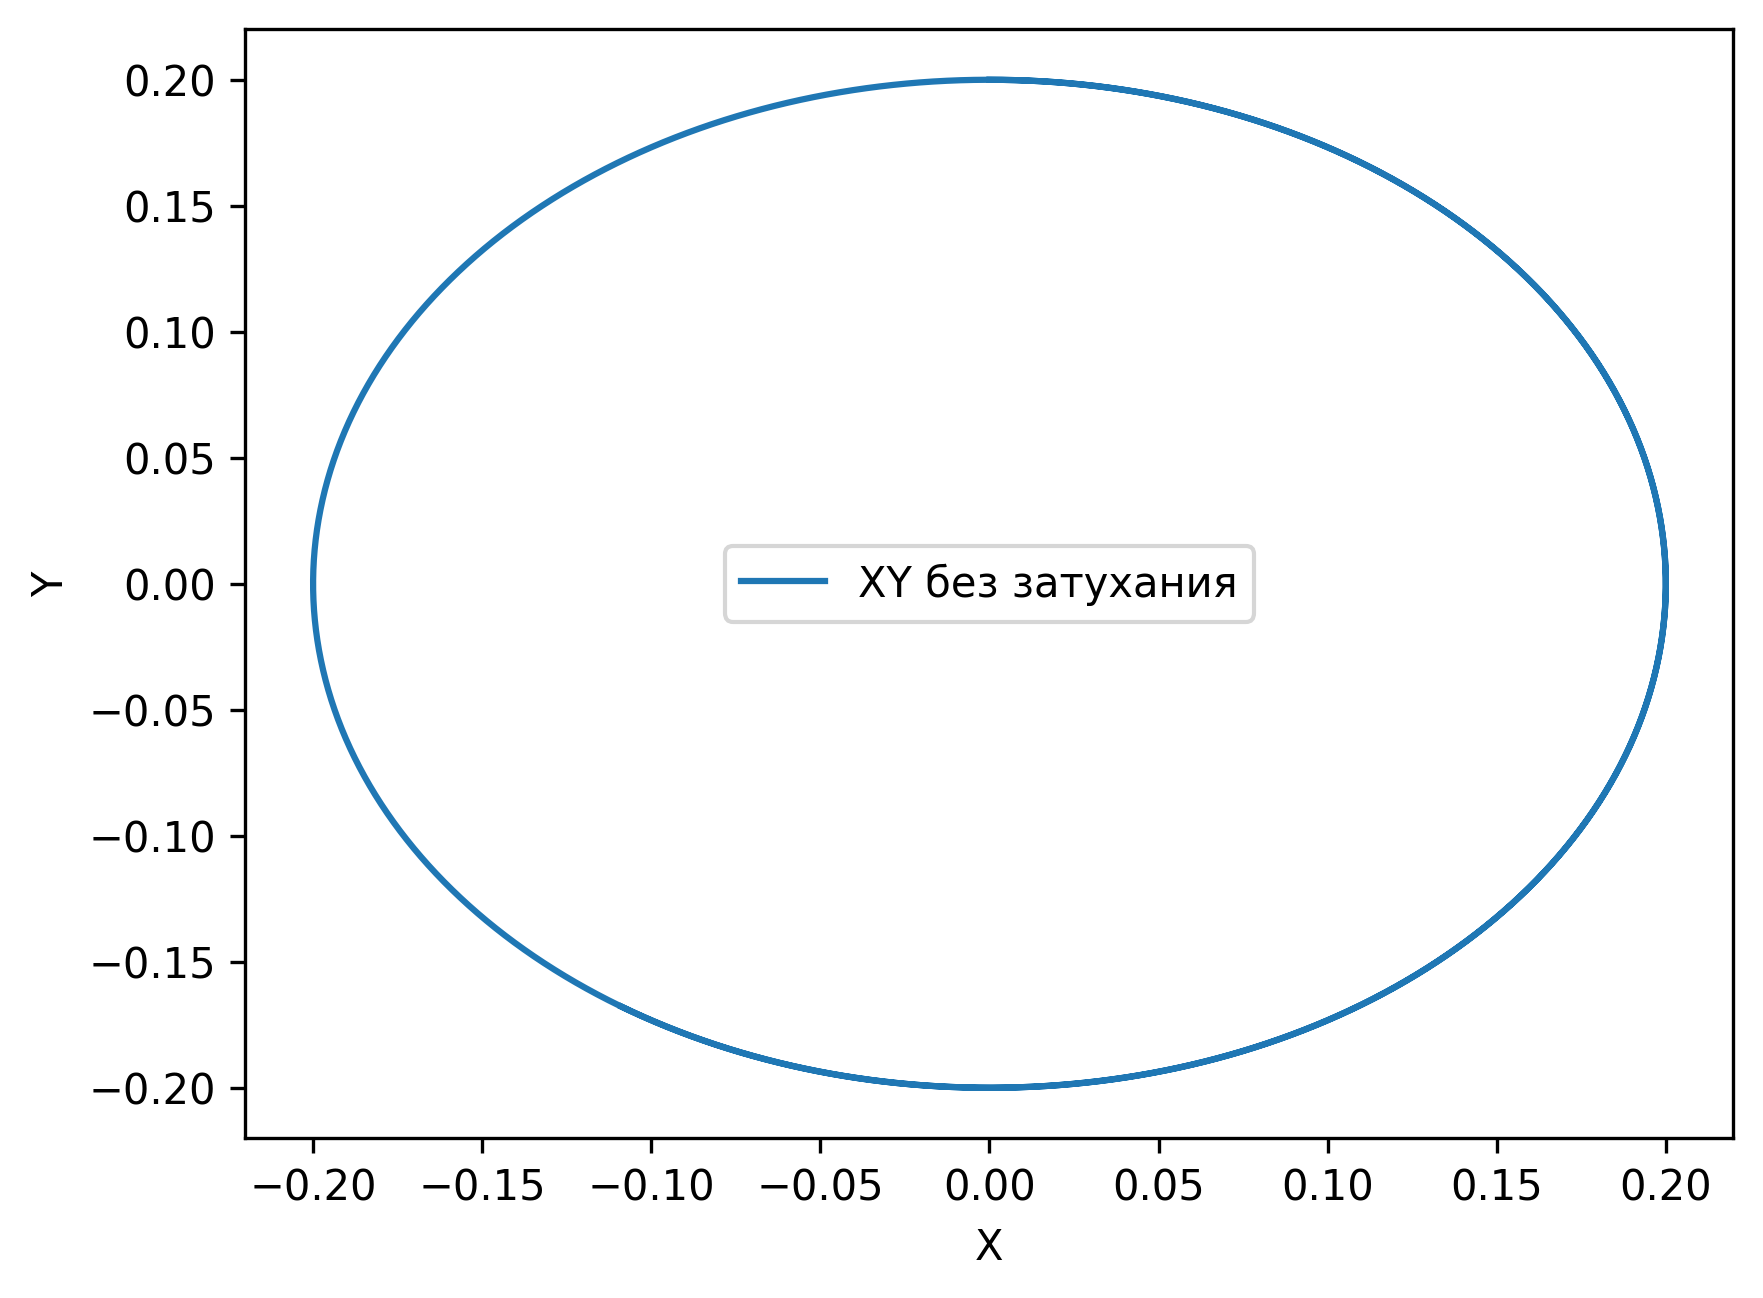
\includegraphics[width=\textwidth]{../pictures/xy_no_damping_omega_0.01.png}
        \captionsetup{font=small}
        \caption*{$\omega_0 = 0{,}01~\text{с}^{-1}$}
    \end{minipage}\hfill
    \begin{minipage}{0.48\textwidth}
        \centering
        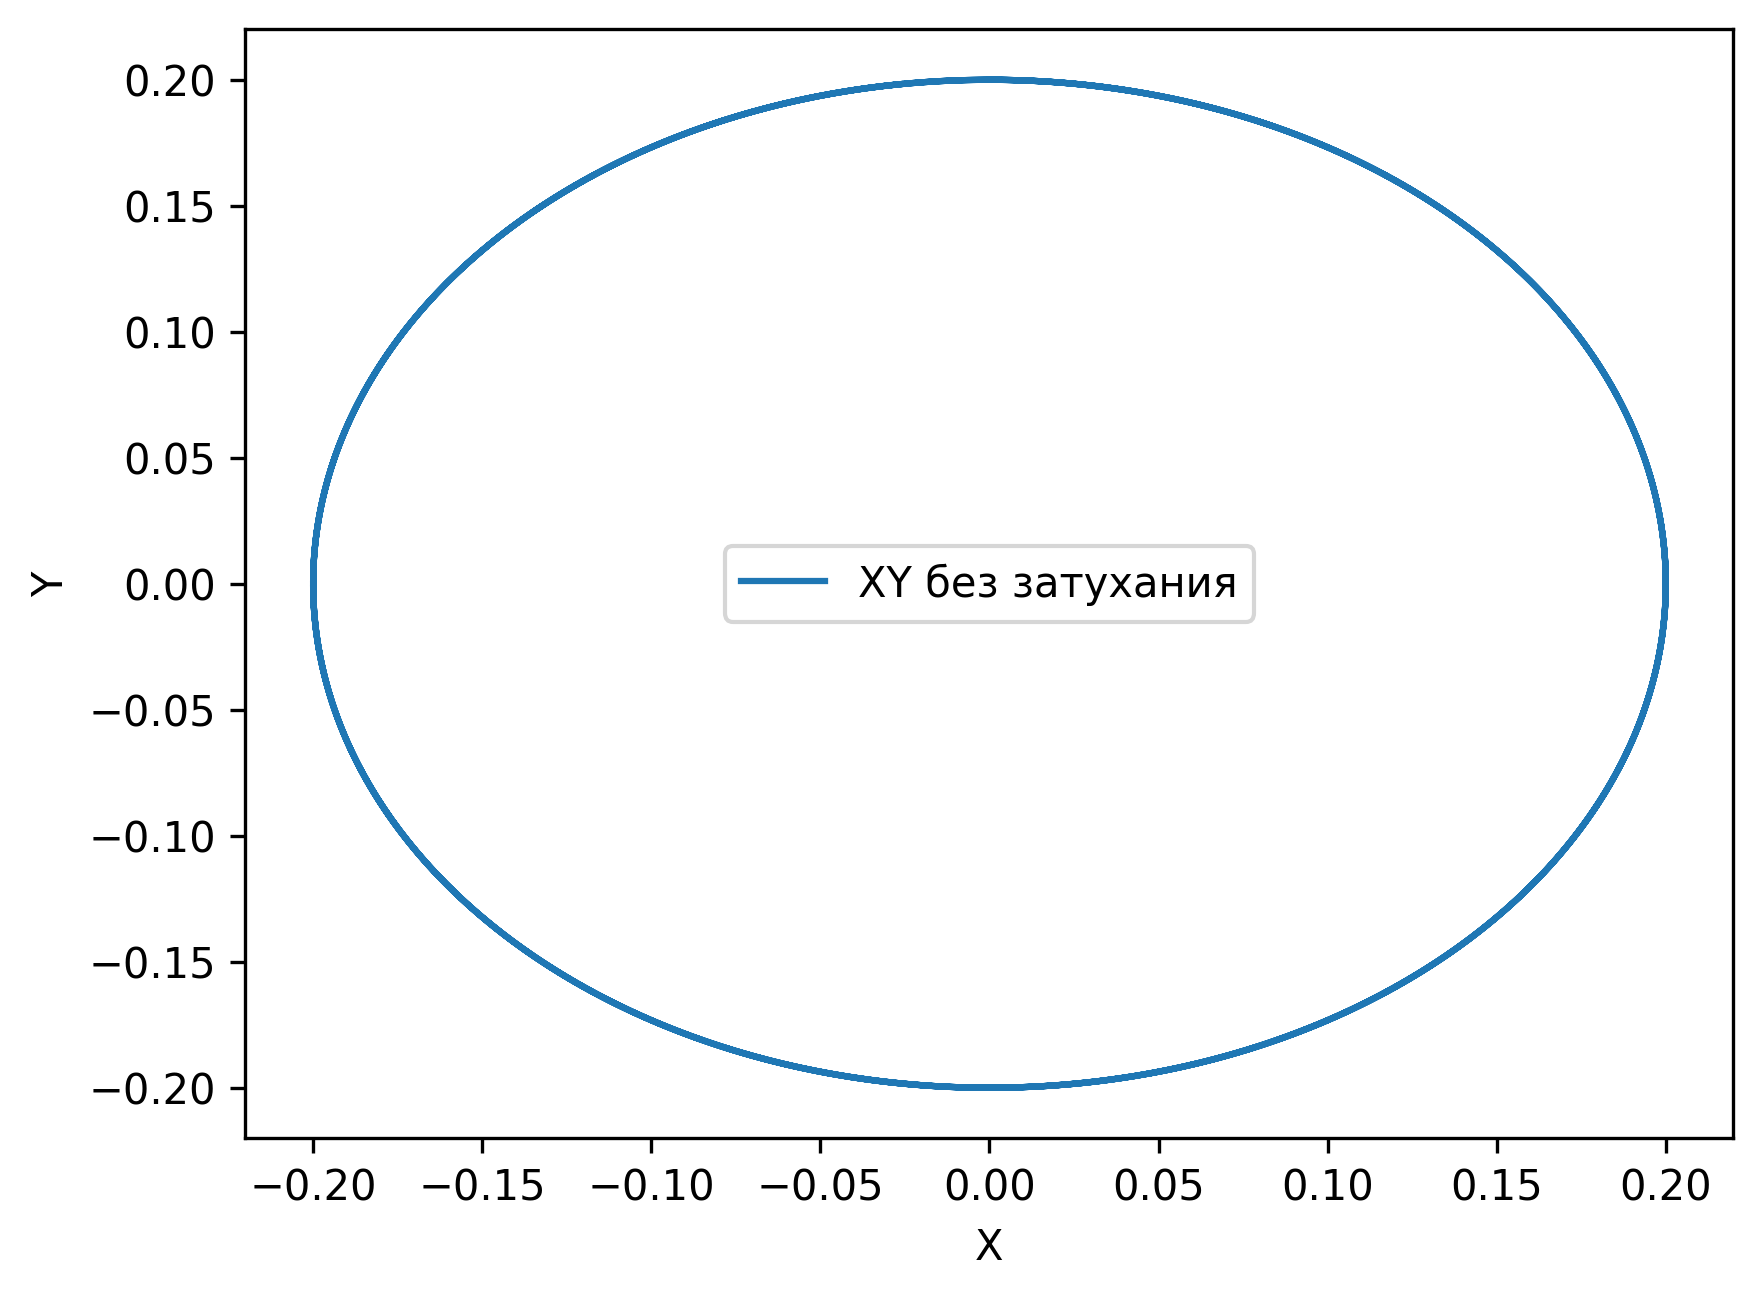
\includegraphics[width=\textwidth]{../pictures/xy_no_damping_omega_0.025.png}
        \caption*{$\omega_0 = 0{,}025~\text{с}^{-1}$}
    \end{minipage}\hfill
    \begin{minipage}{0.48\textwidth}
        \centering
        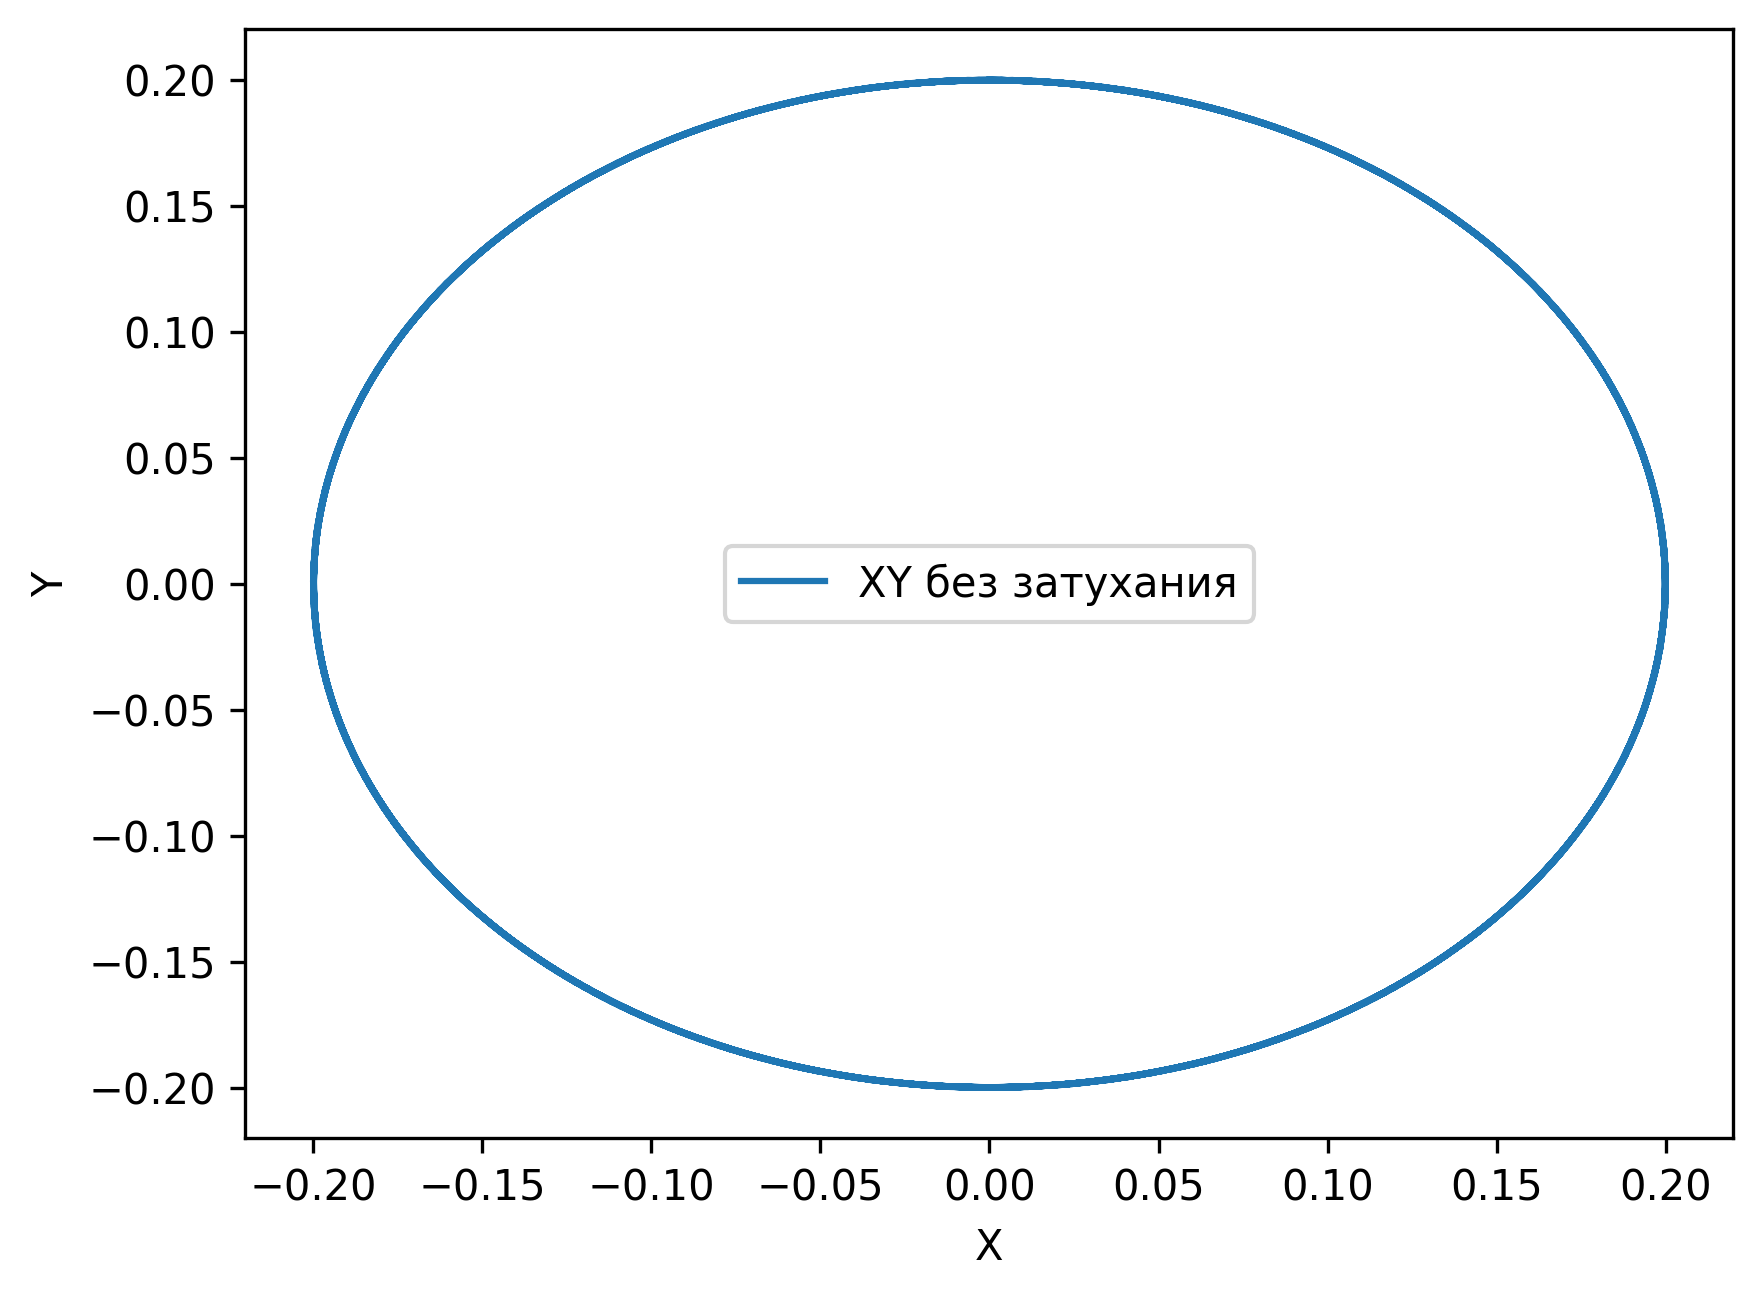
\includegraphics[width=\textwidth]{../pictures/xy_no_damping_omega_0.1.png}
        \caption*{$\omega_0 = 0{,}1~\text{с}^{-1}$}
    \end{minipage}\hfill
    \caption{Траектории маятника на плоскости $XY$ без затухания при различных $\omega_0$}
    \label{fig:xy-no-damping}
\end{figure}

\begin{figure}[H]
    \centering
    \begin{minipage}{0.48\textwidth}
        \centering
        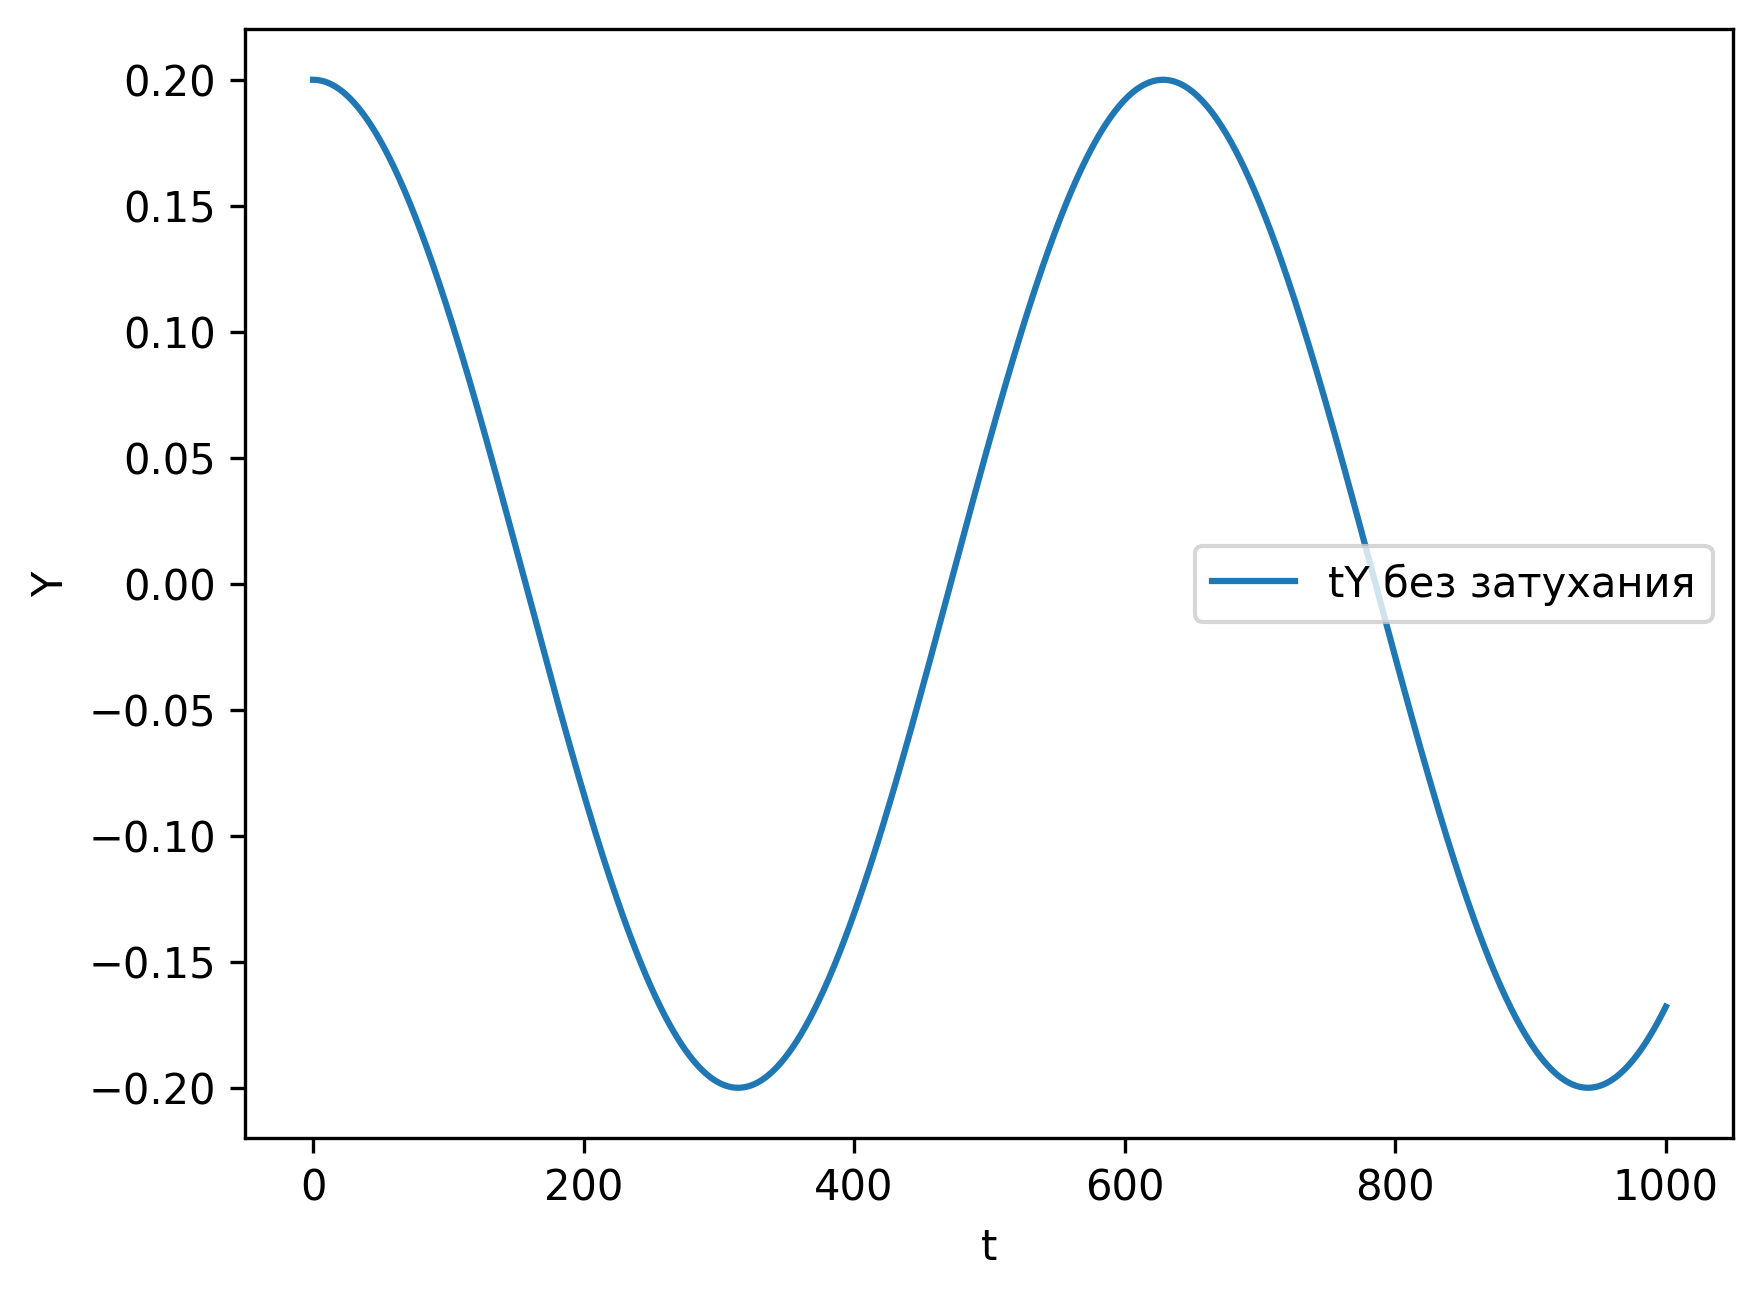
\includegraphics[width=\textwidth]{../pictures/ty_no_damping_omega_0.01.png}
        \caption*{$\omega_0 = 0{,}01~\text{с}^{-1}$}
    \end{minipage}\hfill
    \begin{minipage}{0.48\textwidth}
        \centering
        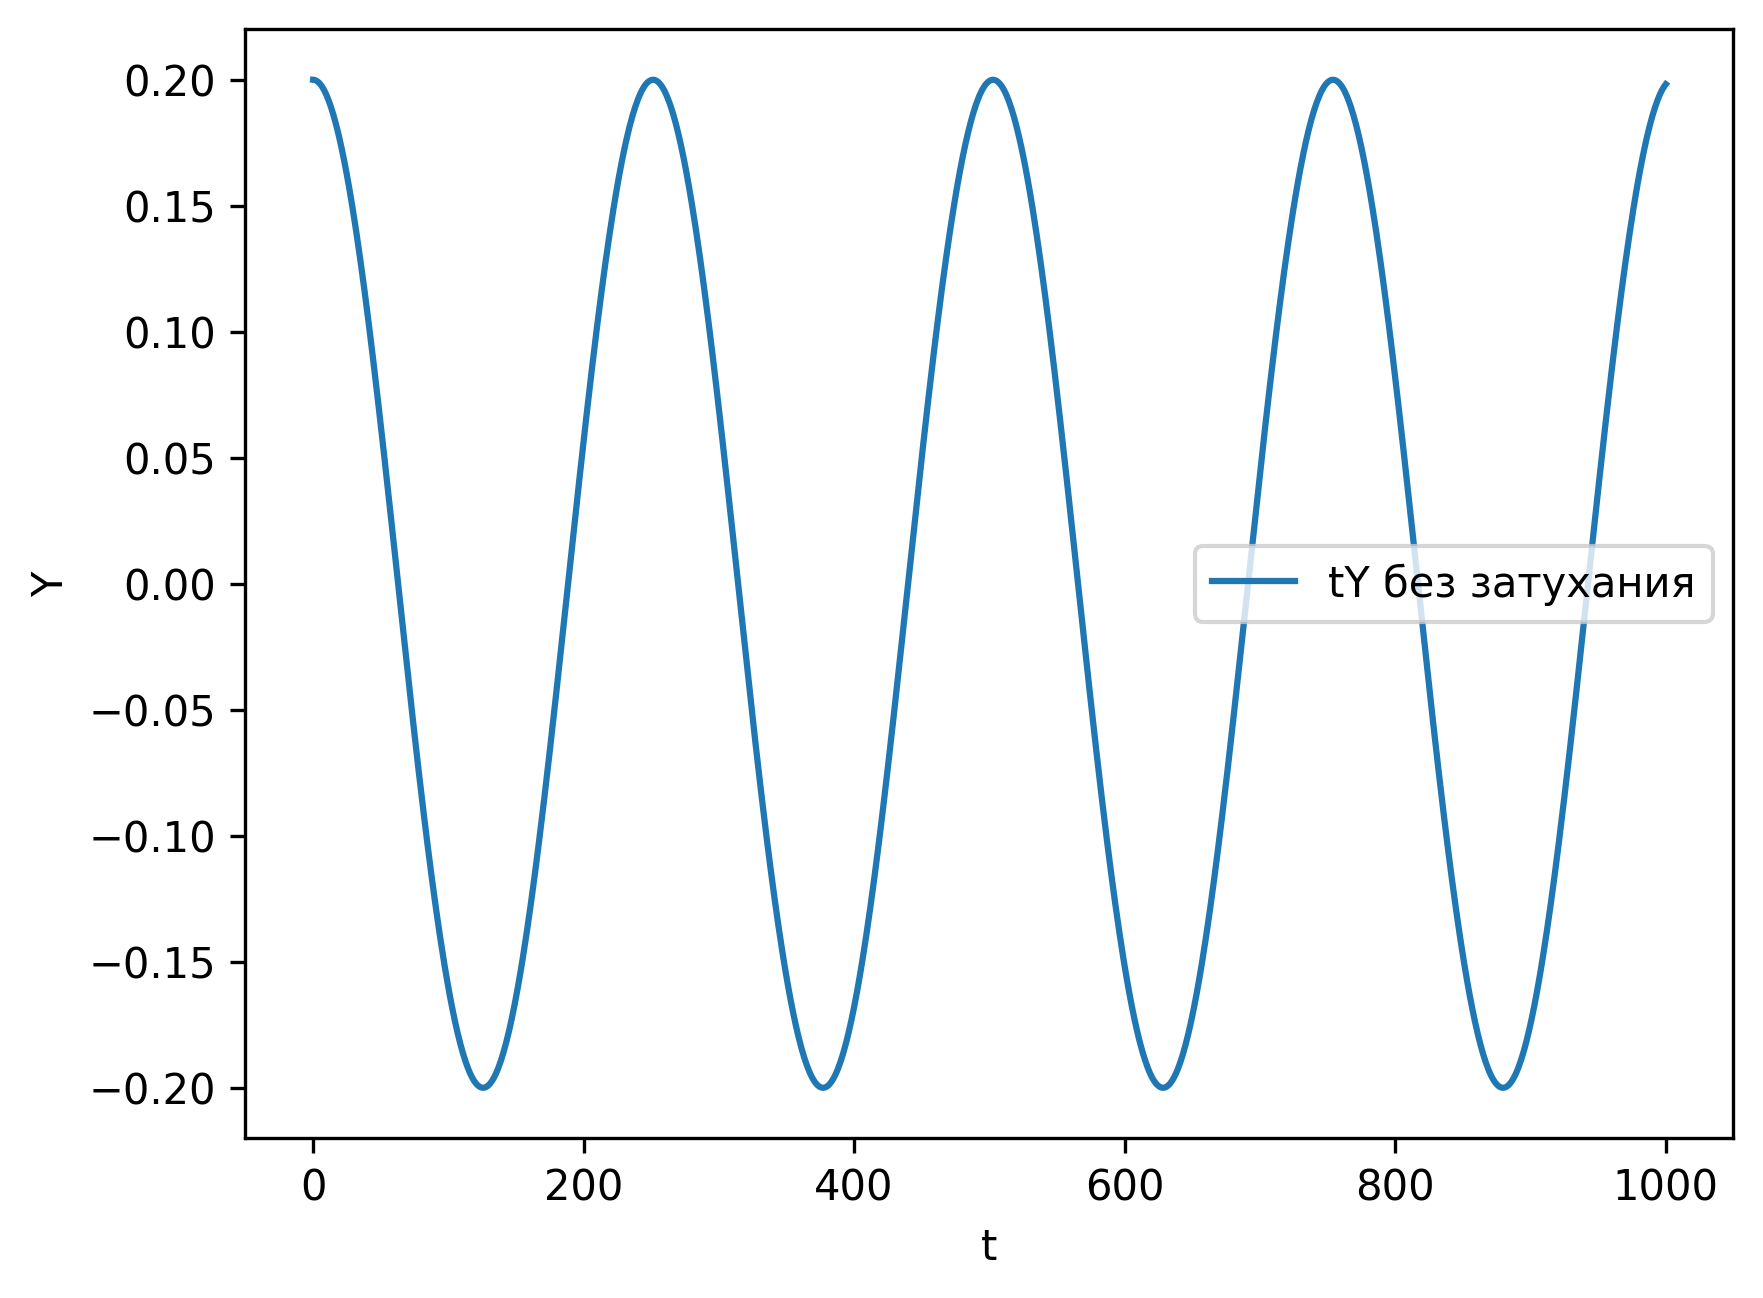
\includegraphics[width=\textwidth]{../pictures/ty_no_damping_omega_0.025.png}
        \caption*{$\omega_0 = 0{,}025~\text{с}^{-1}$}
    \end{minipage}\hfill
    \begin{minipage}{0.48\textwidth}
        \centering
        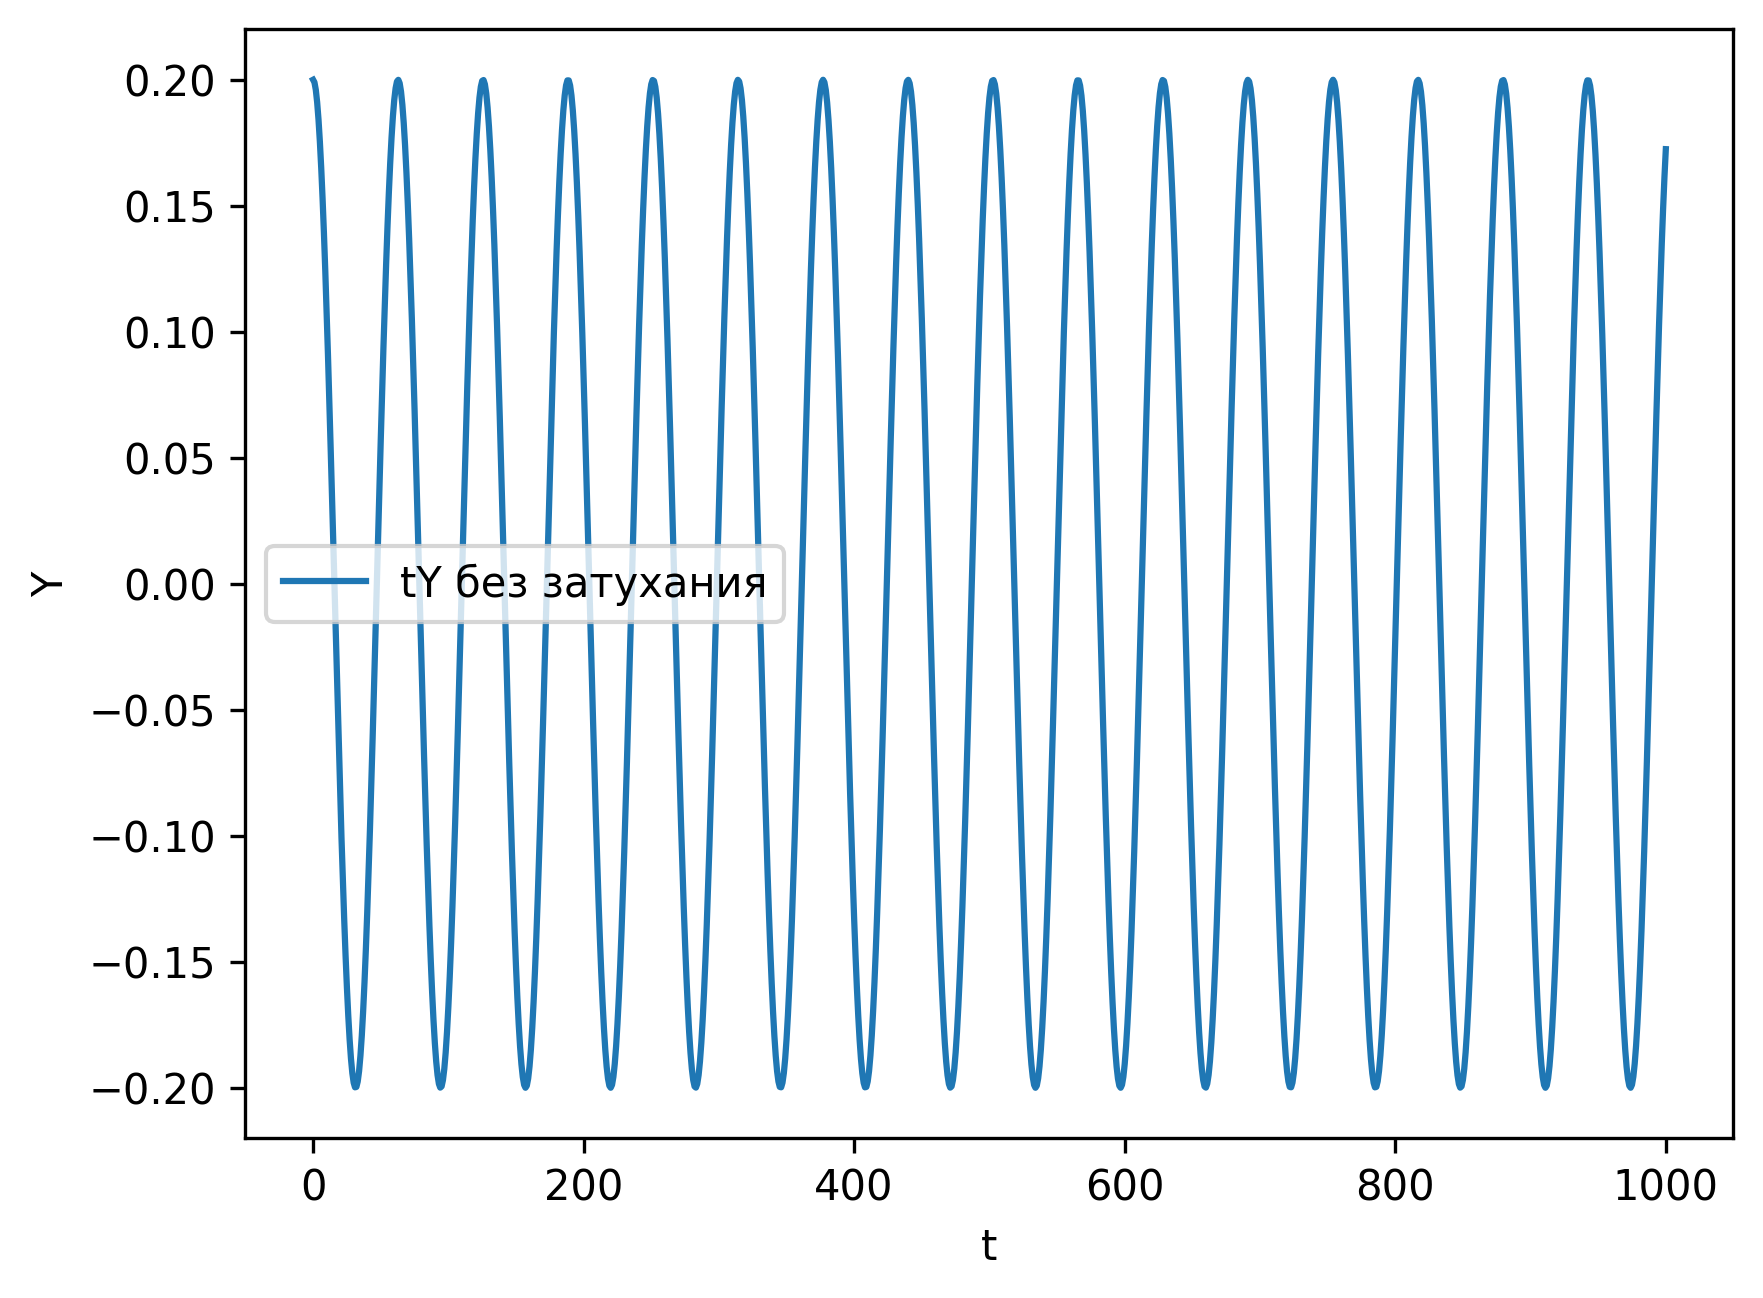
\includegraphics[width=\textwidth]{../pictures/ty_no_damping_omega_0.1.png}
        \caption*{$\omega_0 = 0{,}1~\text{с}^{-1}$}
    \end{minipage}\hfill
    \caption{Зависимость координаты $Y$ от времени без затухания при различных $\omega_0$}
    \label{fig:ty-no-damping}
\end{figure}

\subsectiontext{Затухающие колебания}

При $\sigma = 0{,}01~\text{с}^{-1}$ амплитуда экспоненциально убывает: $A(t) = A_0 e^{-\sigma t}$, так что за время моделирования $t = 1000$~с амплитуда уменьшается примерно в $e^{10} \approx 2 \cdot 10^4$ раз. На графиках $Y(t)$ видны затухающие колебания (рис.~\ref{fig:ty-damping}), а траектории $XY$ представляют собой скручивающиеся спирали, сходящиеся к началу координат (рис.~\ref{fig:xy-damping}).

\begin{figure}[H]
    \centering
    \begin{minipage}{0.48\textwidth}
        \centering
        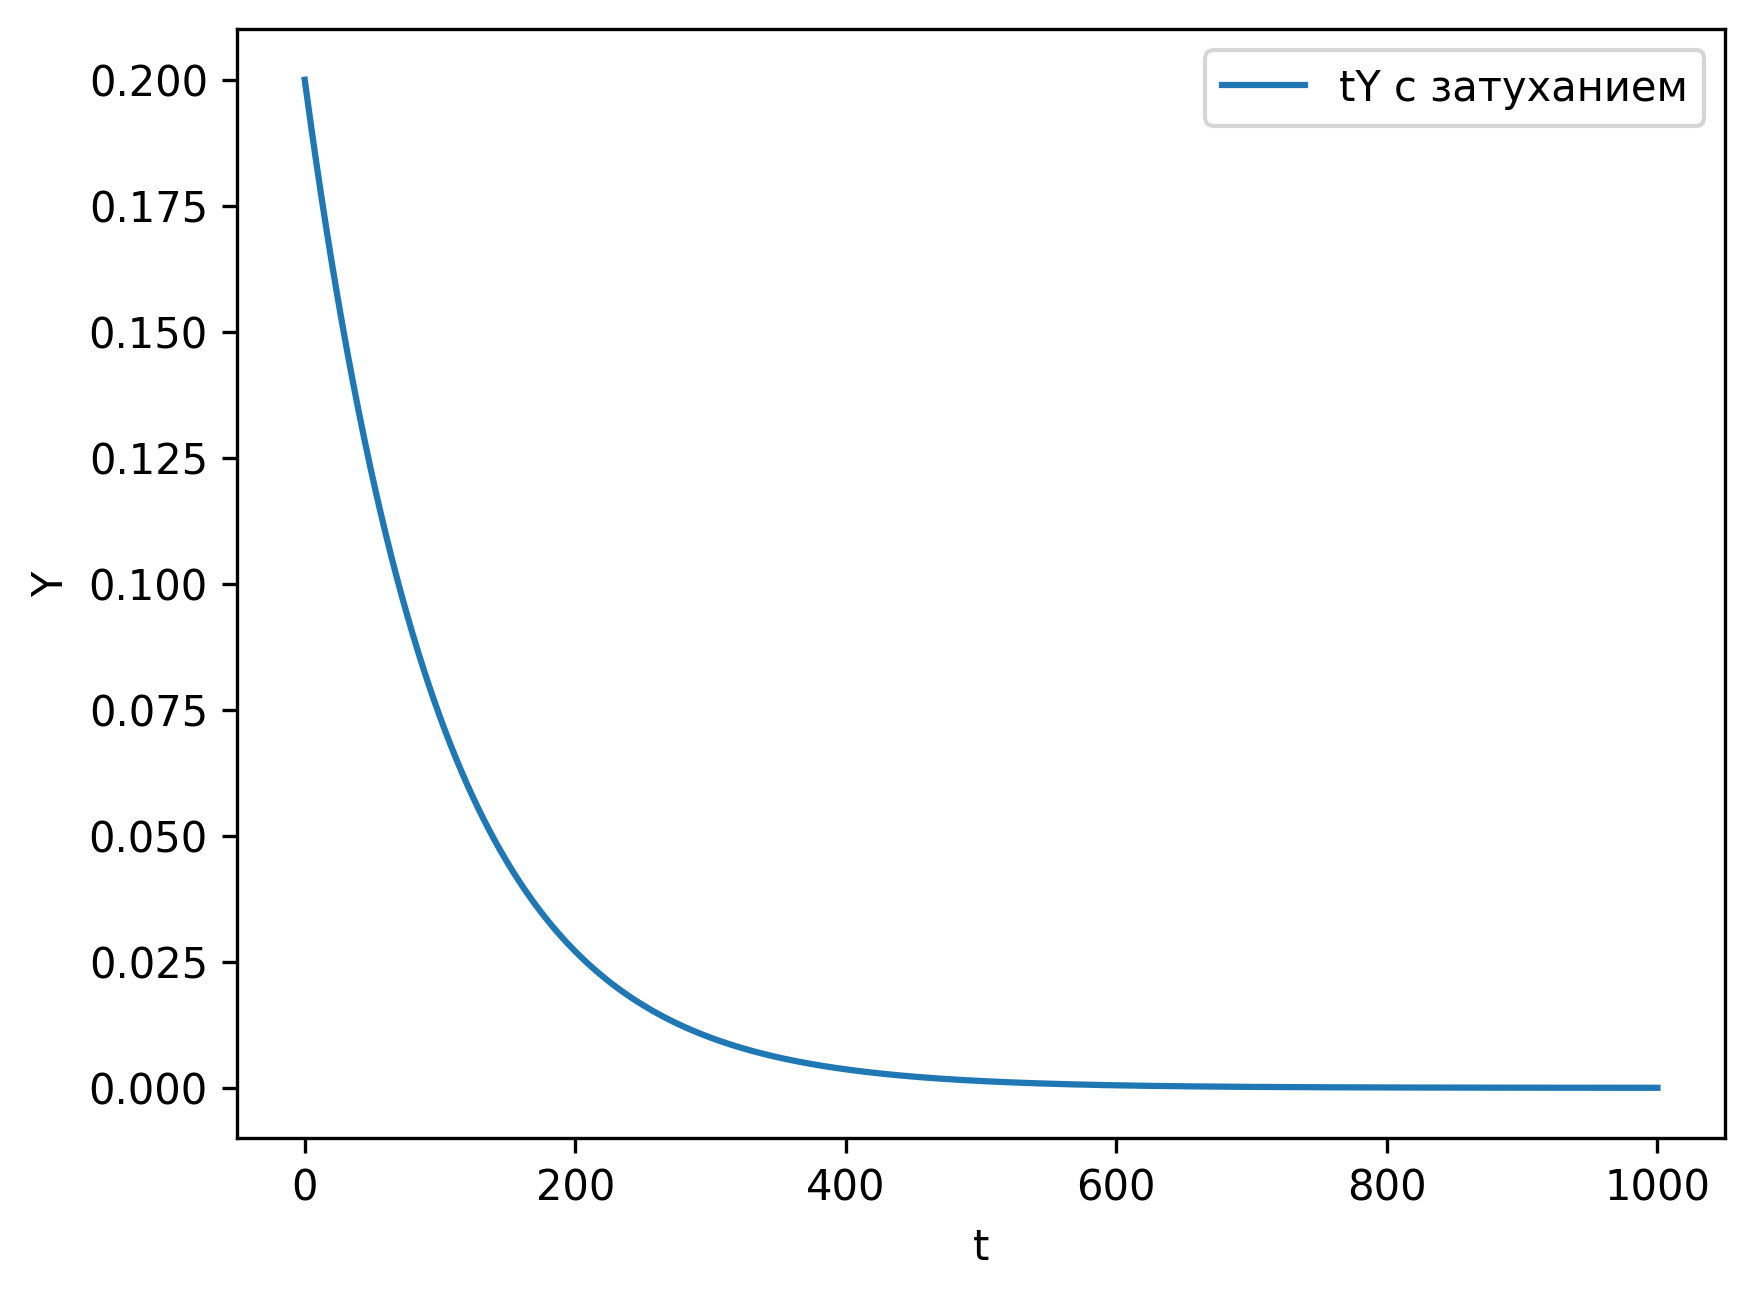
\includegraphics[width=\textwidth]{../pictures/ty_damping_omega_0.01.png}
        \caption*{$\omega_0 = 0{,}01~\text{с}^{-1}$}
    \end{minipage}\hfill
    \begin{minipage}{0.48\textwidth}
        \centering
        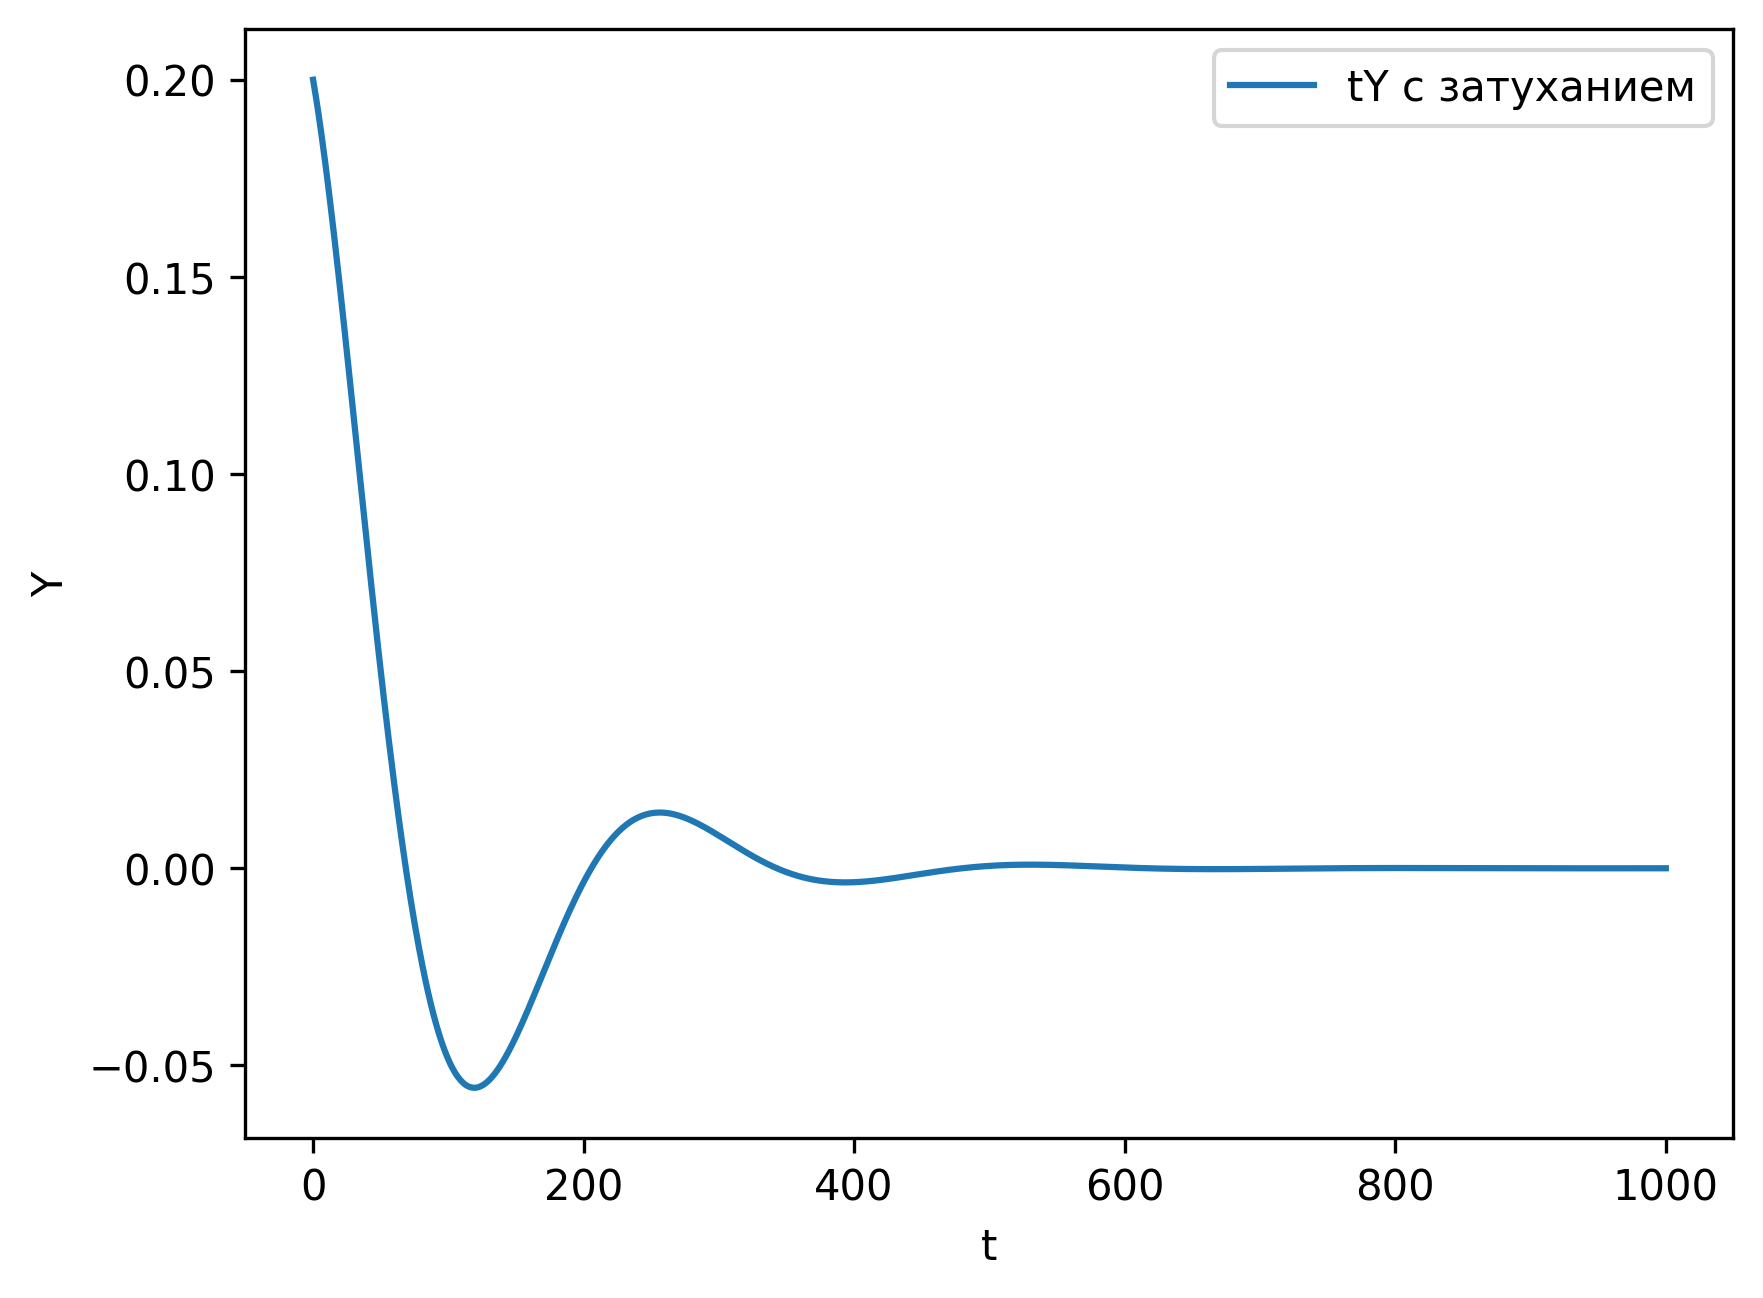
\includegraphics[width=\textwidth]{../pictures/ty_damping_omega_0.025.png}
        \caption*{$\omega_0 = 0{,}025~\text{с}^{-1}$}
    \end{minipage}\hfill
    \begin{minipage}{0.48\textwidth}
        \centering
        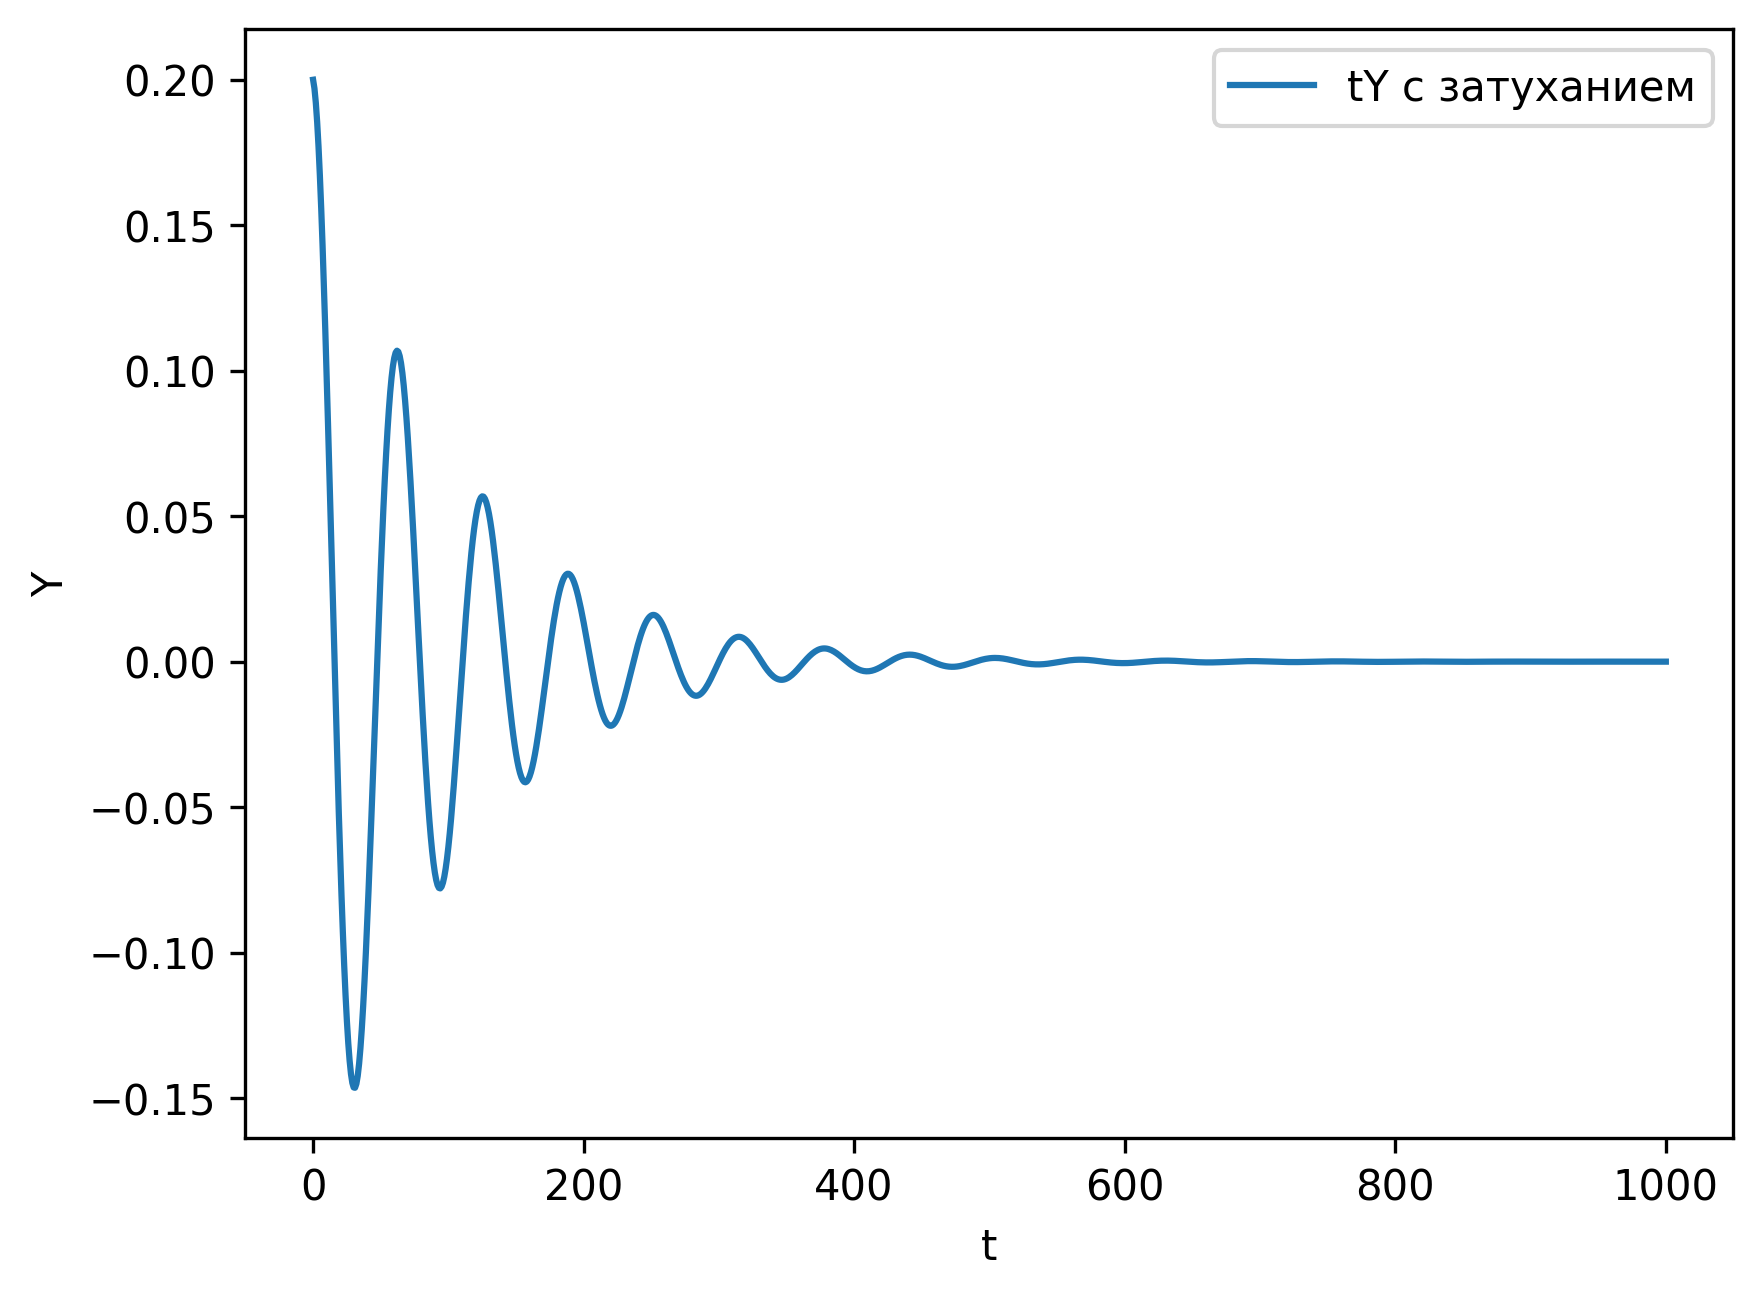
\includegraphics[width=\textwidth]{../pictures/ty_damping_omega_0.1.png}
        \caption*{$\omega_0 = 0{,}1~\text{с}^{-1}$}
    \end{minipage}\hfill
    \caption{Зависимость координаты $Y$ от времени с затуханием при различных $\omega_0$}
    \label{fig:ty-damping}
\end{figure}

\begin{figure}[H]
    \centering
    \begin{minipage}{0.48\textwidth}
        \centering
        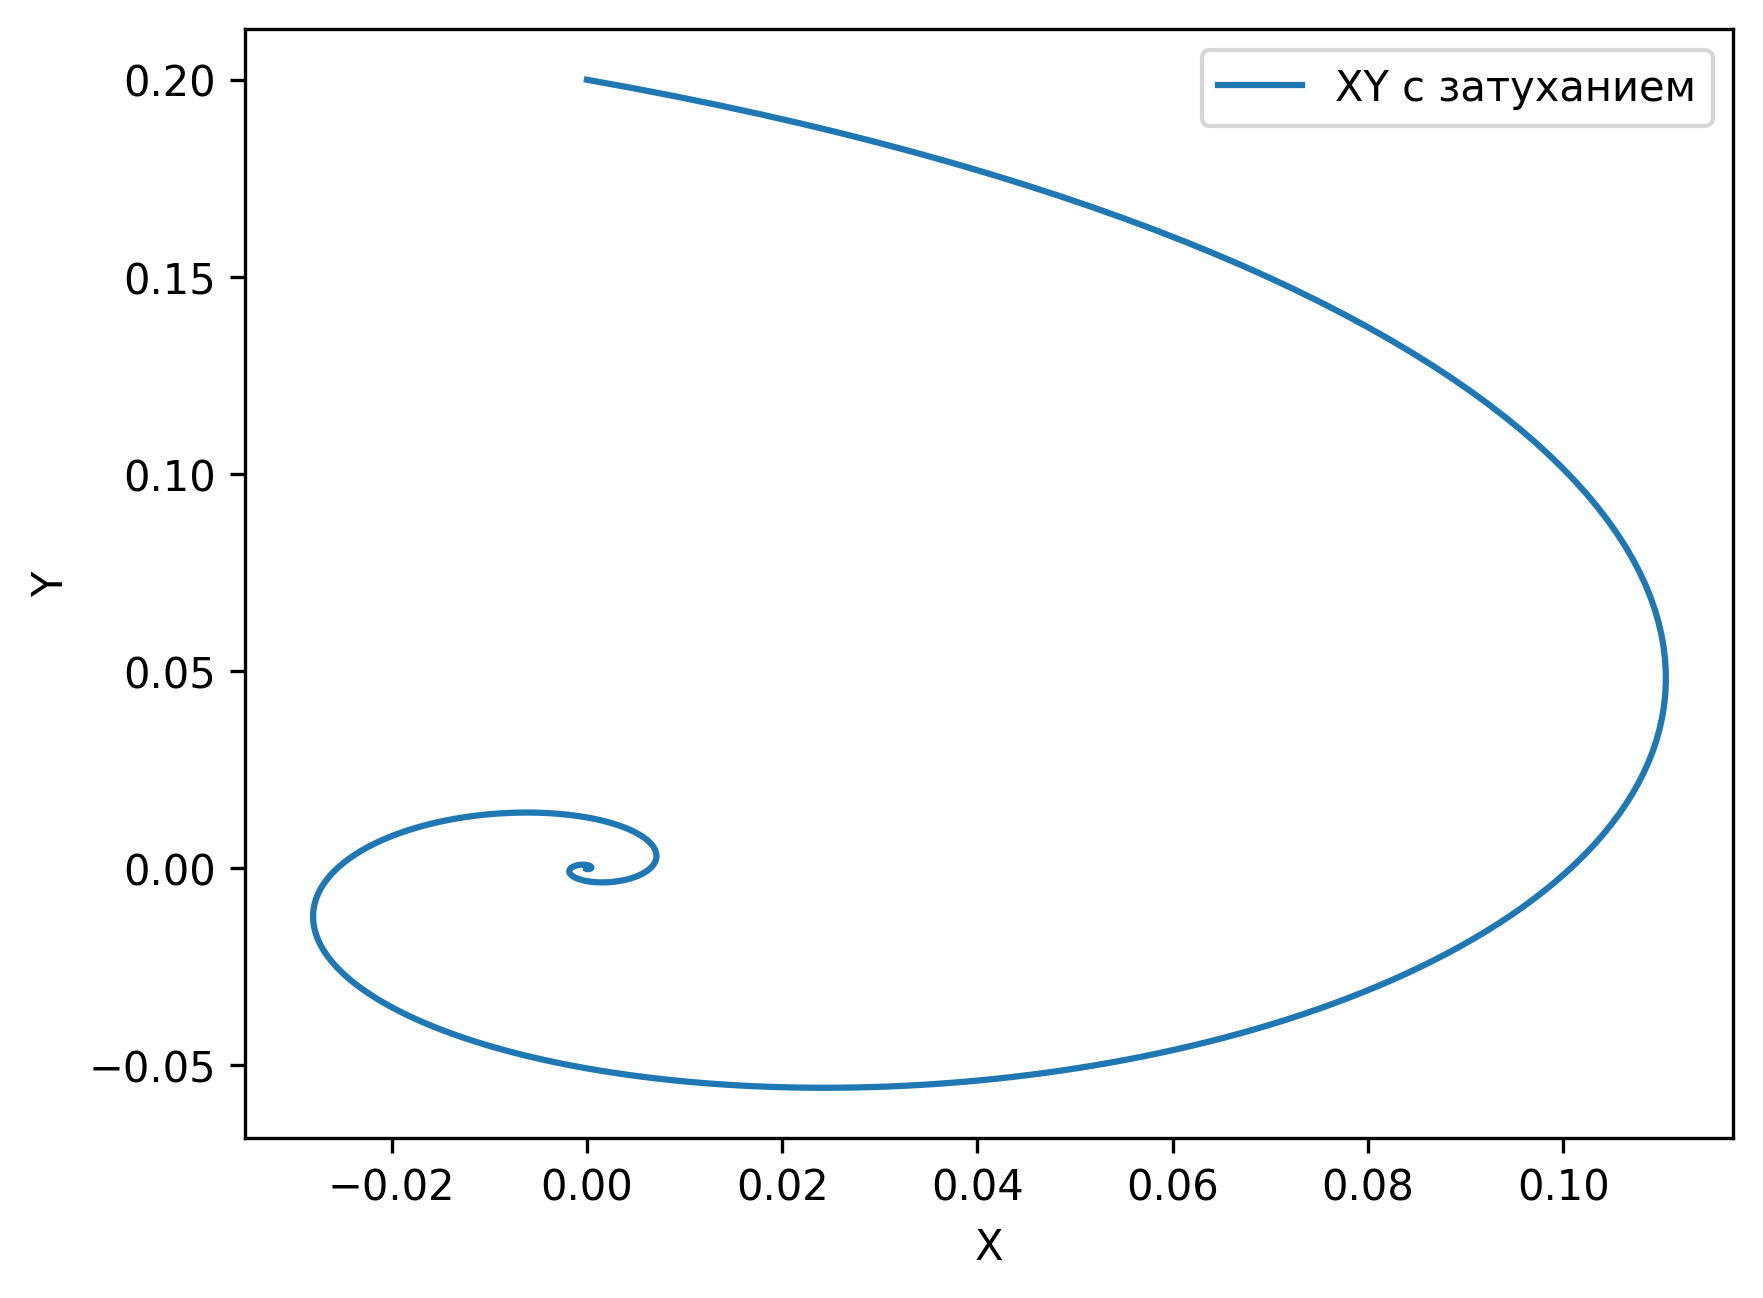
\includegraphics[width=\textwidth]{../pictures/xy_damping_omega_0.025.png}
        \caption*{$\omega_0 = 0{,}025~\text{с}^{-1}$}
    \end{minipage}\hfill
    \begin{minipage}{0.48\textwidth}
        \centering
        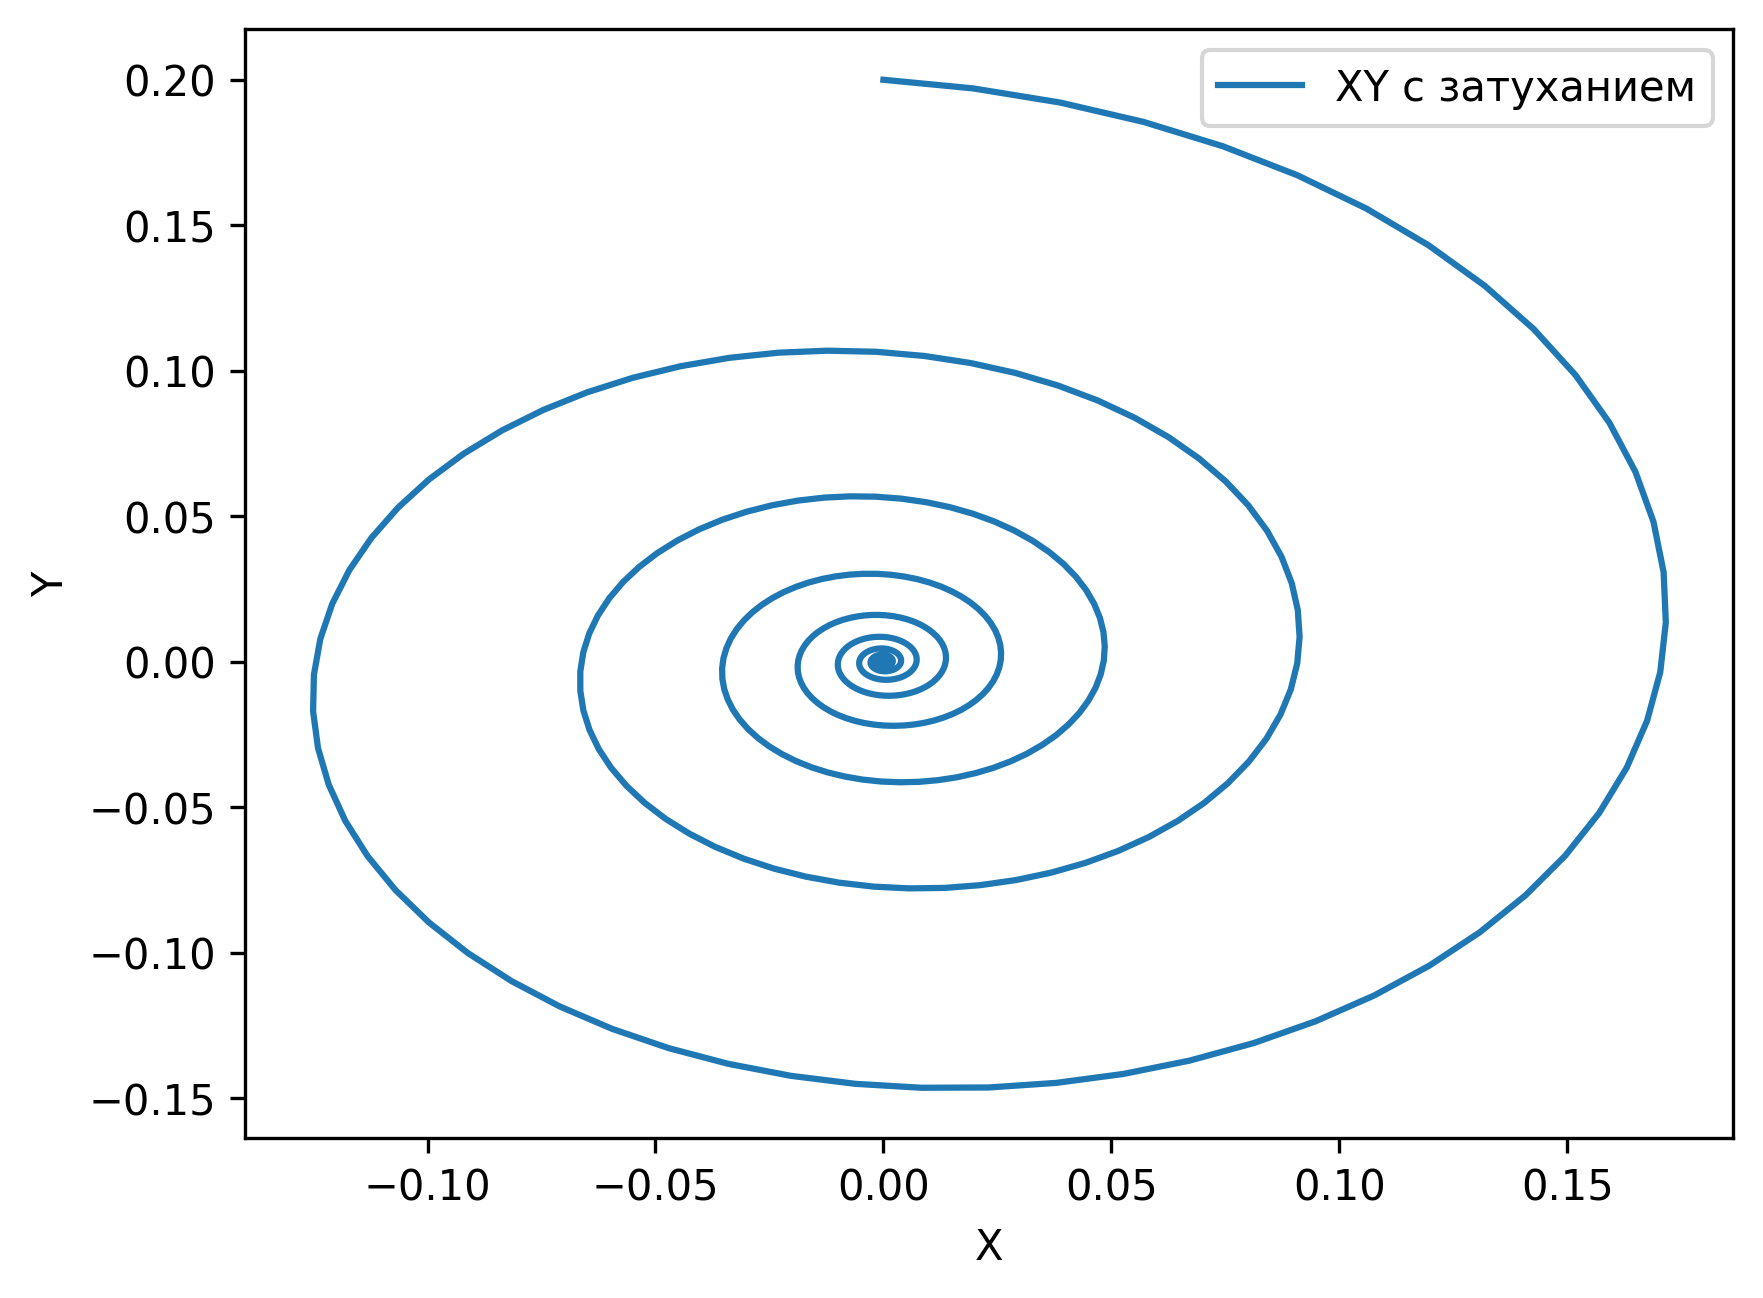
\includegraphics[width=\textwidth]{../pictures/xy_damping_omega_0.1.png}
        \caption*{$\omega_0 = 0{,}1~\text{с}^{-1}$}
    \end{minipage}\hfill
    \begin{minipage}{0.48\textwidth}
        \centering
        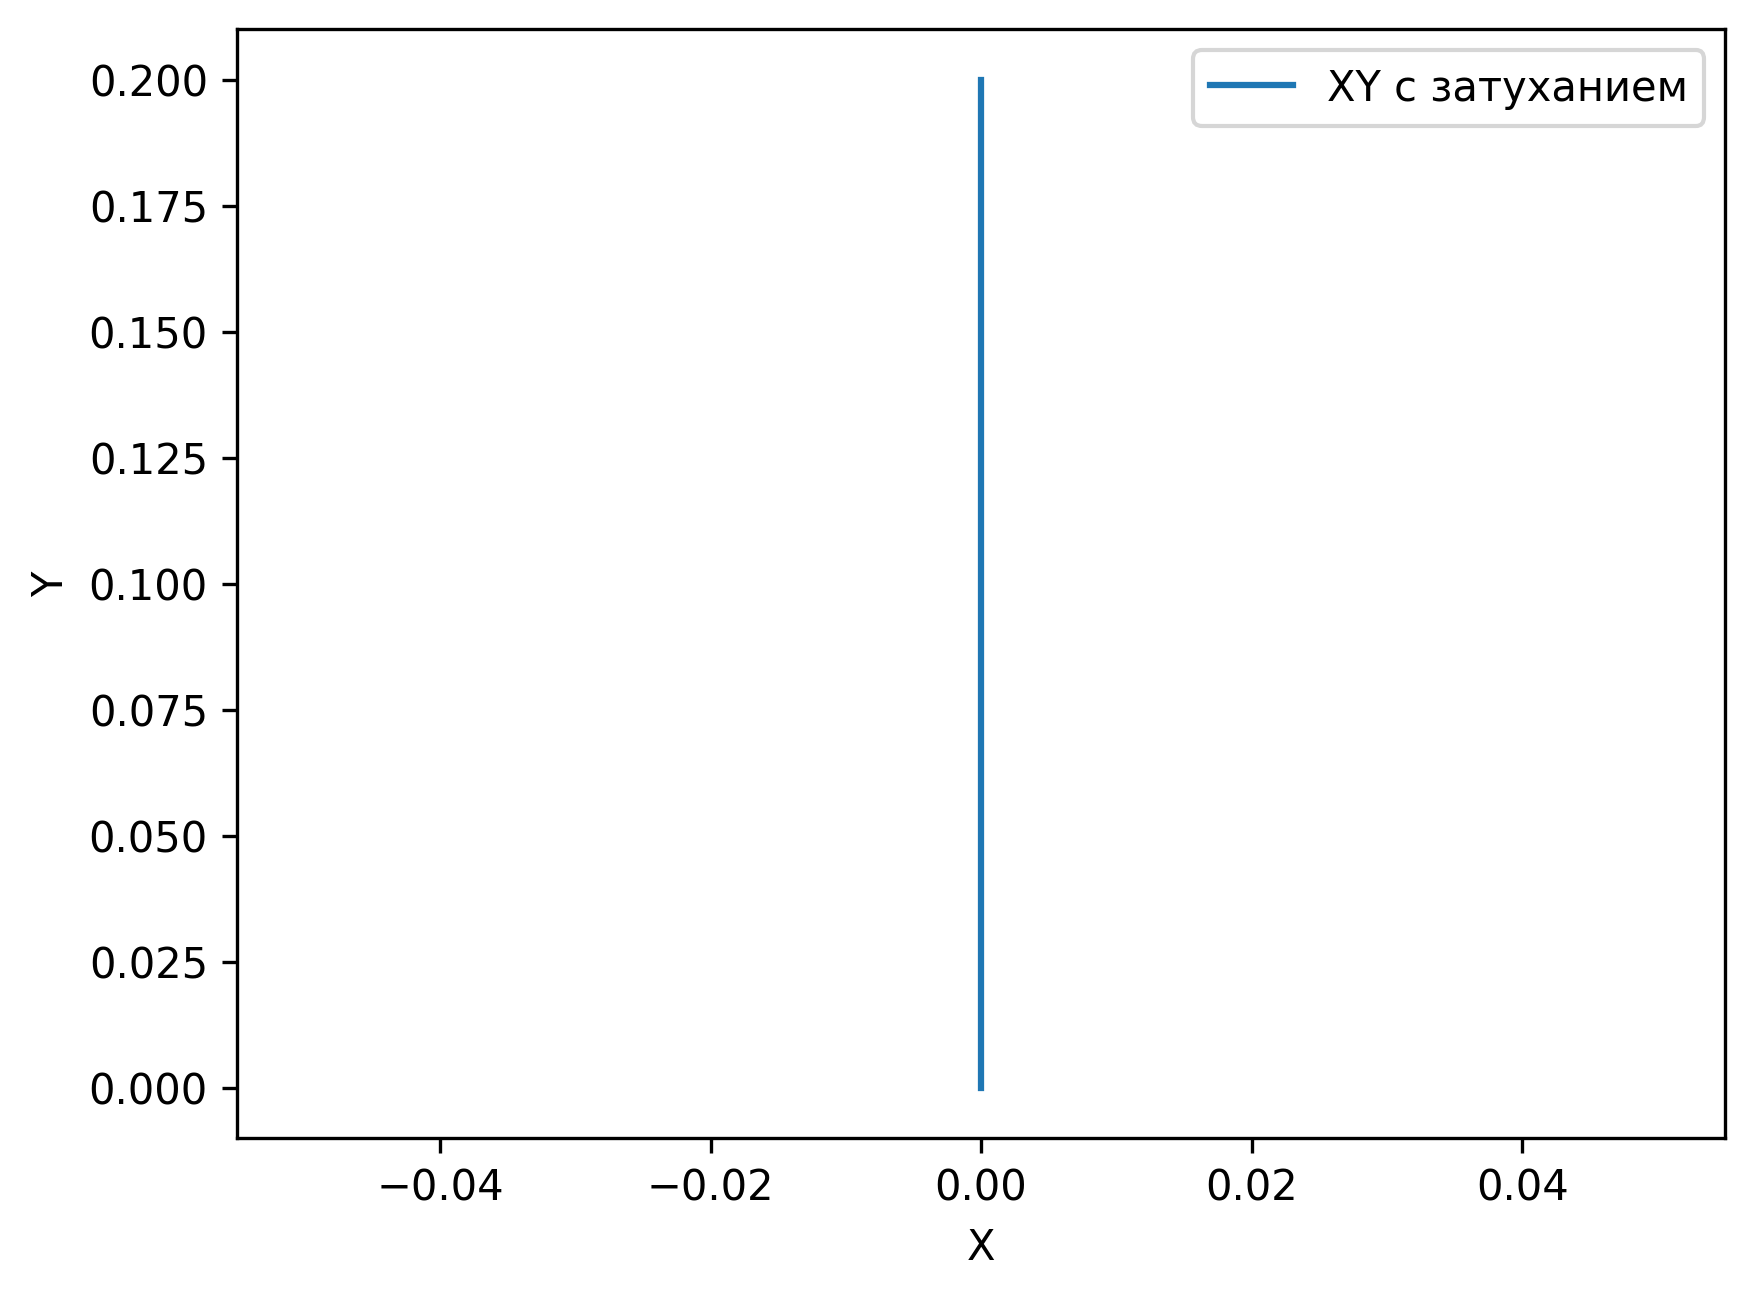
\includegraphics[width=\textwidth]{../pictures/xy_damping_omega_0.01.png}
        \caption*{$\omega_0 = 0{,}01~\text{с}^{-1}$}
    \end{minipage}\hfill
    \caption{Траектории маятника на плоскости $XY$ с затуханием при различных $\omega_0$. Особый случай: при $\omega_0 = 0{,}01~\text{с}^{-1}$ вместо спирали наблюдается вертикальная линия}
    \label{fig:xy-damping}
\end{figure}

\subsectiontext{Особый случай: вырождение колебаний при $\omega_0 = \sigma$}

Для $\omega_0 = 0{,}01~\text{с}^{-1}$ и $\sigma = 0{,}01~\text{с}^{-1}$ выполняется равенство $\omega_0 = \sigma$, поэтому частота затухающих колебаний $\omega = \sqrt{\omega_0^2 - \sigma^2} = 0$. Колебания полностью вырождаются: маятник без колебаний экспоненциально возвращается в положение равновесия. Поскольку начальная фаза $\varphi = 0$, координата $x(t) = A_0 e^{-\sigma t} \sin 0 \equiv 0$, а $y(t) = A_0 e^{-\sigma t}$ монотонно убывает от $A_0$ до нуля. В результате на плоскости $XY$ вместо скручивающейся спирали наблюдается вертикальная линия вдоль оси $Y$ (нижний график на рис.~\ref{fig:xy-damping}), что соответствует граничному (критическому) режиму затухания.

\newpage

% --- Вывод ---
\mainsection{Вывод}
\label{sec:conclusion}

В работе исследованы колебания математического маятника, описываемые моделью гармонического осциллятора, для случаев отсутствия и наличия затухания при различных собственных частотах $\omega_0 = 0{,}01$; $0{,}025$; $0{,}1~\text{с}^{-1}$.

Получены следующие результаты:
\begin{itemize}
    \item без затухания маятник совершает гармонические колебания с постоянной амплитудой $A_0 = 0{,}2$~м, а его траектория на плоскости $XY$ является окружностью радиуса $A_0$;
    \item при затухании $\sigma = 0{,}01~\text{с}^{-1}$ амплитуда колебаний экспоненциально убывает по закону $A(t) = A_0 e^{-\sigma t}$, а траектория на плоскости $XY$ имеет вид скручивающейся спирали, сходящейся к началу координат;
    \item в особом случае $\omega_0 = \sigma$ (при $\omega_0 = 0{,}01~\text{с}^{-1}$) частота затухающих колебаний обращается в нуль, колебания вырождаются в апериодическое движение, и вместо спирали на плоскости $XY$ наблюдается вертикальная линия, что соответствует критическому режиму затухания.
\end{itemize}

Результаты численного расчёта полностью согласуются с теорией затухающих колебаний.

\end{document}